%% vrst2026.tex — ACM VRST 2026 full paper
%% Markerless Mixed-Reality Injection Training on Commodity Headsets.
%%
%% SUBMISSION/REVIEW NOTE:
%%  - For double-blind review (confirm VRST 2026 review model on the CFP), switch the
%%    documentclass line to:  \documentclass[sigconf,review,anonymous]{acmart}
%%    and comment out the \author/\affiliation/\email block (acmart inserts "Anonymous Author(s)").
%%  - This draft uses [sigconf] so authors can read it with names visible.
%%
\documentclass[sigconf]{acmart}

\AtBeginDocument{%
  \providecommand\BibTeX{{%
    Bib\TeX}}}

%% Architecture diagram (vector, no external image needed).
\usepackage{tikz}
\usetikzlibrary{positioning,arrows.meta,fit,backgrounds}

%% --- Placeholder figure helper: renders a labelled grey box so the paper COMPILES
%% --- without any image files. Replace each \figplaceholder with \includegraphics
%% --- once the real screenshots/charts exist.
\newcommand{\figplaceholder}[2]{%
  \fcolorbox{black}{black!8}{\parbox[c][#1][c]{0.97\linewidth}{\centering\small\itshape
  [PLACEHOLDER]\\ #2}}}

%% Rights / conference metadata (SAMPLE values — replace from the ACM rights email).
\setcopyright{acmlicensed}
\copyrightyear{2026}
\acmYear{2026}
\acmDOI{XXXXXXX.XXXXXXX}
\acmConference[VRST '26]{32nd ACM Symposium on Virtual Reality Software and Technology}{November 16--18, 2026}{Sendai, Japan}
\acmISBN{978-1-4503-XXXX-X/2026/11}

\begin{document}

\title{Markerless Mixed-Reality Injection Training on Commodity Headsets:
Real-Time 3D Geometric Guidance for Needle Angle and Depth}

%% Author block (comment out for anonymous review — see note at top of file).
\author{Divijh Mangtani}
\authornote{Both authors contributed equally to this research.}
\email{divijh.mangtani@research.iiit.ac.in}
\orcid{1234-5678-9012}
\affiliation{%
  \institution{Software Engineering Research Center, IIIT Hyderabad}
  \city{Hyderabad}
  \country{India}}

\author{Vijay Arvaynthan S R}
\authornotemark[1]
\correspondingauthor
\email{vijay.s@research.iiit.ac.in}
\orcid{0009-0006-0099-5839}
\affiliation{%
  \institution{Software Engineering Research Center, IIIT Hyderabad}
  \city{Hyderabad}
  \country{India}}

\author{Y. Raghu Reddy}
\email{raghu.reddy@iiit.ac.in}
\affiliation{%
  \institution{Software Engineering Research Center, IIIT Hyderabad}
  \city{Hyderabad}
  \country{India}}

\renewcommand{\shortauthors}{Mangtani et al.}

\begin{abstract}
Safe injection technique---correct entry angle, insertion depth, and steadiness---is a
high-volume clinical skill that benefits from repeated, low-risk practice. Existing virtual- and
mixed-reality (MR) needle-insertion trainers achieve high fidelity with haptic devices,
instrumented props, and external trackers, but this hardware raises cost and setup burden and
limits deployment to a handful of equipped labs. We present a \emph{markerless, hardware-free}
MR injection trainer that runs entirely on a consumer standalone headset (Meta Quest~3). The
system reconstructs a virtual syringe from articulated hand tracking and overlays \emph{real-time
3D geometric guidance} on a learner-placed injection site: a colour-coded cone of valid entry
angles specific to the chosen injection type (intramuscular, subcutaneous, intradermal,
intravenous) and stacked depth zones (correct, too-deep, maximum) that the needle must respect.
To counter the angle and depth error introduced by finger occlusion of the held syringe, we
introduce a \emph{center-snap} pose model that anchors the needle entry to the target site and
derives angle from a long, stable lever. The trainer scores each attempt on angle, depth, speed,
flow, and removal stability. We describe the system architecture and a study protocol that
evaluates accuracy (angle error, depth error, tip-to-center distance, completion time) and
usability (SUS, NASA-TLX) with and without the guidance overlay.
\textbf{[PLACEHOLDER RESULTS: insert headline findings after the study is run.]}
\end{abstract}

\begin{CCSXML}
<ccs2012>
 <concept>
  <concept_id>10003120.10003123.10010860</concept_id>
  <concept_desc>Human-centered computing~Mixed / augmented reality</concept_desc>
  <concept_significance>500</concept_significance>
 </concept>
 <concept>
  <concept_id>10003120.10003123.10011748</concept_id>
  <concept_desc>Human-centered computing~Empirical studies in HCI</concept_desc>
  <concept_significance>300</concept_significance>
 </concept>
 <concept>
  <concept_id>10010405.10010497.10010500</concept_id>
  <concept_desc>Applied computing~Health informatics</concept_desc>
  <concept_significance>300</concept_significance>
 </concept>
 <concept>
  <concept_id>10010405.10010489.10010490</concept_id>
  <concept_desc>Applied computing~Interactive learning environments</concept_desc>
  <concept_significance>100</concept_significance>
 </concept>
</ccs2012>
\end{CCSXML}

\ccsdesc[500]{Human-centered computing~Mixed / augmented reality}
\ccsdesc[300]{Human-centered computing~Empirical studies in HCI}
\ccsdesc[300]{Applied computing~Health informatics}
\ccsdesc[100]{Applied computing~Interactive learning environments}

\keywords{mixed reality, hand tracking, medical simulation, injection training,
needle insertion, visual guidance, standalone HMD, Meta Quest}

\begin{teaserfigure}
  \figplaceholder{4.5cm}{Teaser: in-headset view of the markerless injection trainer. A virtual
  syringe (reconstructed from hand tracking), the learner-placed injection site, the blue
  valid-angle cone for the selected injection type, and the green/red/orange depth zones below the
  skin. Replace with a composite passthrough capture.}
  \caption{The markerless MR injection trainer running on a standalone Meta Quest~3. No haptic
  device, instrumented prop, or external tracker is used.}
  \Description{A mixed reality scene showing a hand holding a virtual syringe over a target site
  with a coloured guidance cone and depth zones.}
  \label{fig:teaser}
\end{teaserfigure}

\maketitle

\section{Introduction}
Parenteral injection is among the most frequently performed clinical procedures, and poor
technique---wrong entry angle, shallow or excessive depth, or an unsteady hand---contributes to
pain, tissue damage, and failed delivery. Competence is built through repetition, but live
practice is constrained by patient safety, consumables, and supervisor availability. Simulation
addresses this gap, and virtual reality (VR) training has repeatedly transferred to improved
real-world performance in adjacent procedural skills~\cite{seymour2002vr}.

Most VR/MR needle trainers pursue \emph{physical fidelity}: they couple a head-mounted display
with haptic devices, instrumented syringes, or electromagnetically tracked tools so that learners
feel tissue resistance and manipulate a real object
~\cite{kim2023bimanual,guruge2025acupuncture,yang2026multimodal}. This fidelity is valuable, but
the hardware is expensive, requires per-session calibration across coordinate systems, and ties
the experience to a small number of equipped labs. The result is a training modality that scales
poorly to the large, distributed populations---nursing and medical students, community health
workers---who most need volume practice.

We take the opposite design stance and ask how much useful injection-technique training can be
delivered with \emph{no added hardware at all}: a single consumer standalone headset, markerless
articulated hand tracking, and software. Rather than reproduce haptic sensation, we make the
\emph{geometry of a correct injection explicit and continuously visible}. The learner pinches to
place an injection site; the system reconstructs a virtual syringe from their hand and renders, in
3D and in real time, (i)~a cone of acceptable entry angles whose aperture is specific to the
selected injection type, and (ii)~stacked depth zones---correct, too-deep, and a maximum-depth
floor---that the needle tip must respect (Figure~\ref{fig:teaser}). Each attempt is scored on
angle, insertion depth and speed, plunger flow rate, and withdrawal stability.

A core technical obstacle is that the hand holding a syringe \emph{occludes the very fingers used
to infer the tool's pose}, so a na\"ively reconstructed needle axis and tip jitter badly. We
contribute a \emph{center-snap} pose model: because the learner is always aiming at the placed
site, we anchor the needle's entry point to the site center and derive the syringe angle from the
long, stable lever between that anchor and the hand, which is far less sensitive to fingertip
noise than the short, occluded needle segment.

\medskip\noindent\textbf{Contributions.}
\begin{itemize}
  \item A markerless, hardware-free MR injection-technique trainer that runs entirely on a
  commodity standalone HMD, lowering the cost and setup barrier of prior haptic/instrumented
  systems.
  \item A real-time 3D geometric guidance design---per-injection-type valid-angle cones and
  colour-coded depth zones---that externalizes the clinical targets for angle and depth.
  \item A center-snap pose model that makes hand-tracked angle and depth estimation robust to the
  finger occlusion inherent in holding a virtual syringe.
  \item A study protocol and \textbf{[PLACEHOLDER: results]} evaluating accuracy and usability,
  with and without guidance.
\end{itemize}

\section{Related Work}
\subsection{VR and MR needle-insertion training}
Needle and injection trainers have been a recurring target for immersive simulation. Recent
systems emphasize haptic realism: \citet{kim2023bimanual} integrate two heterogeneous haptic
devices with a HoloLens~2 for bimanual intravenous insertion, varying skin and vein properties,
and evaluate with 20 participants (9 experts, 11 novices) using the NASA-TLX. \citet{guruge2025acupuncture}
combine MR with haptic feedback for acupuncture needling. These works deliver convincing tactile
cues but depend on specialized devices and multi-coordinate calibration. Our system deliberately
forgoes haptics to remain deployable on unmodified consumer hardware, trading tactile fidelity for
accessibility and continuous \emph{visual} guidance.

\subsection{Hand tracking and tool guidance}
Markerless articulated hand tracking is now standard on consumer headsets, enabling controller-free
interaction but introducing jitter and occlusion when the hand grips a tool. Mixed-reality
procedural simulators have used external cameras and spatial co-registration to track hands
together with instrumented tools~\cite{spatialtutor2024}, and multimodal approaches add wrist-based
vibrotactile cues to AR overlays for handheld-tool guidance~\cite{yang2026multimodal}. We instead
reconstruct the tool purely from on-device hand joints and address occlusion in software via the
center-snap model.

\subsection{Guidance cues and scoring metrics}
Needle-training systems commonly report composite accuracy from normalized metrics---insertion
depth, angular deviation, tip-to-center distance, and task duration---and contrast novice and
expert performance. Depth-responsive visual guidance has been shown to reduce mean depth error and
task time in MR needle tasks. Our guidance makes these same target quantities (angle window, depth
band, entry point) \emph{directly visible as 3D geometry} rather than as numeric read-outs, and our
scoring adopts the established angle/depth/time metrics so results are comparable to prior work.

\subsection{Positioning}
Table~\ref{tab:related} contrasts representative systems on hardware, headset class, feedback
modality, and accessibility. To our knowledge, ours is the first injection-technique trainer that
combines markerless hand-tracked tool reconstruction, per-type 3D geometric guidance, and on-device
scoring on a single commodity standalone HMD with no added hardware.

\begin{table*}[t]
  \centering
  \caption{Representative needle/injection trainers vs.\ our system. \textbf{[PLACEHOLDER: verify
  each cell against the cited source before camera-ready.]}}
  \label{tab:related}
  \begin{tabular}{llllc}
    \toprule
    System & Headset / display & Tool tracking & Feedback & Added hardware \\
    \midrule
    Kim et al.~\cite{kim2023bimanual} & HoloLens 2 (MR) & Haptic gloves + stylus & Haptic + visual & Yes (high) \\
    Guruge et al.~\cite{guruge2025acupuncture} & MR display & Instrumented & Haptic + visual & Yes (high) \\
    Yang et al.~\cite{yang2026multimodal} & AR & Tracked handheld tool & Wrist haptic + AR & Yes (moderate) \\
    SpatialTutor~\cite{spatialtutor2024} & MR + external cameras & CV + co-registration & Visual & Yes (moderate) \\
    \textbf{Ours} & \textbf{Quest 3 (standalone)} & \textbf{Markerless hand tracking} & \textbf{3D visual guidance} & \textbf{None} \\
    \bottomrule
  \end{tabular}
\end{table*}

\section{System}
\subsection{Architecture}
The trainer is built in Unity and runs as a standalone Android application on Meta Quest~3 via
OpenXR and the Unity XR Hands subsystem; mixed-reality passthrough places the virtual content in
the user's real environment. The runtime is organized as a small set of cooperating components
(Figure~\ref{fig:arch}): \textsf{SyringeOverlayTracker} reconstructs the syringe from hand joints;
\textsf{SurfaceSelectionTool} captures the injection site from pinch gestures;
\textsf{InjectionTargetGuide} renders the 3D guidance; \textsf{SyringeCalibrationButtonBridge}
holds the per-type clinical profiles and computes the per-attempt metrics and score; and
\textsf{GoalManager} orchestrates the guided workflow and the floating coaching UI. No physical
syringe, marker, or external sensor is used.

\begin{figure*}[t]
  \centering
  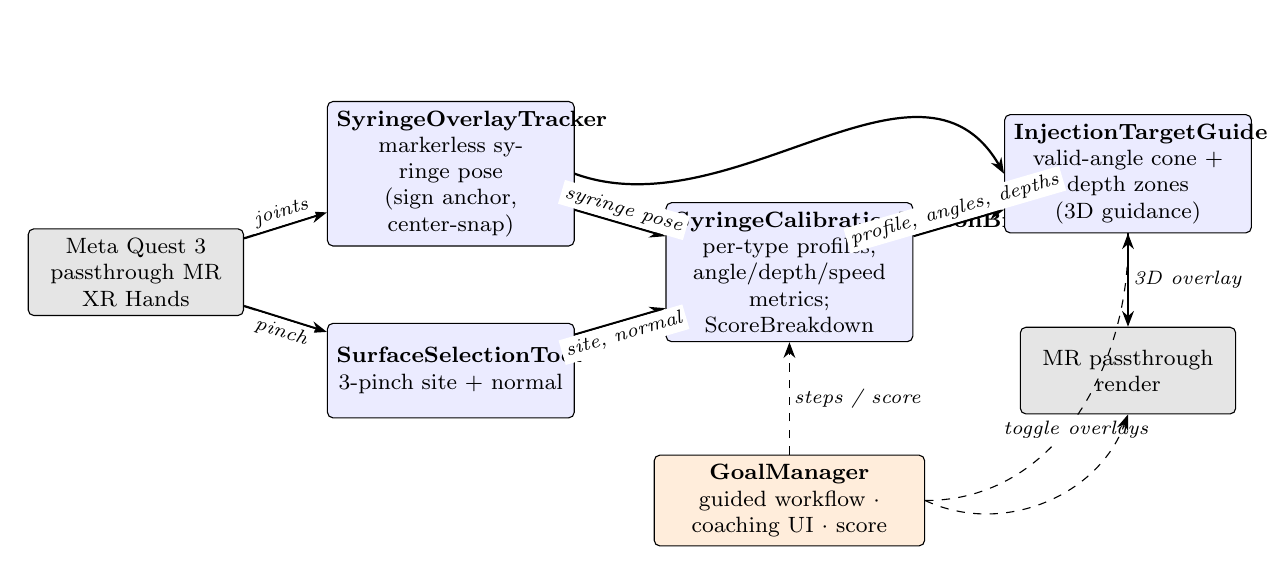
\begin{tikzpicture}[
    font=\footnotesize,
    io/.style={draw, rounded corners=2pt, fill=black!10, align=center,
               text width=2.5cm, minimum height=11mm},
    comp/.style={draw, rounded corners=2pt, fill=blue!8, align=center,
                 text width=2.9cm, minimum height=12mm},
    orch/.style={draw, rounded corners=2pt, fill=orange!14, align=center,
                 text width=3.2cm, minimum height=10mm},
    flow/.style={-{Stealth[length=2mm]}, thick},
    ctrl/.style={-{Stealth[length=2mm]}, dashed},
    elbl/.style={font=\scriptsize\itshape, fill=white, inner sep=1.5pt}]

    \node[io]   (sensor)  at (0,0)      {Meta Quest~3\\passthrough MR\\XR Hands};
    \node[comp] (tracker) at (4,1.25)   {\textbf{SyringeOverlayTracker}\\markerless syringe pose\\(sign anchor, center-snap)};
    \node[comp] (surface) at (4,-1.25)  {\textbf{SurfaceSelectionTool}\\3-pinch site + normal};
    \node[comp] (bridge)  at (8.3,0)    {\textbf{SyringeCalibrationButtonBridge}\\per-type profiles;\\angle/depth/speed metrics;\\ScoreBreakdown};
    \node[comp] (guide)   at (12.6,1.25){\textbf{InjectionTargetGuide}\\valid-angle cone +\\depth zones (3D guidance)};
    \node[io]   (display) at (12.6,-1.25){MR passthrough\\render};
    \node[orch] (goal)    at (8.3,-2.9) {\textbf{GoalManager}\\guided workflow $\cdot$ coaching UI $\cdot$ score};

    \draw[flow] (sensor) -- node[elbl,above,sloped]{joints} (tracker);
    \draw[flow] (sensor) -- node[elbl,below,sloped]{pinch} (surface);
    \draw[flow] (tracker) -- node[elbl,above,sloped]{syringe pose} (bridge);
    \draw[flow] (surface) -- node[elbl,below,sloped]{site, normal} (bridge);
    \draw[flow] (bridge) -- node[elbl,above,sloped]{profile, angles, depths} (guide);
    \draw[flow] (guide) -- node[elbl,right]{3D overlay} (display);
    \draw[flow] (tracker.east) to[out=-20,in=120] (guide.west);

    \draw[ctrl] (goal) -- node[elbl,right]{steps / score} (bridge);
    \draw[ctrl] (goal.east) to[out=0,in=-90] node[elbl,below]{toggle overlays} (guide.south);
    \draw[ctrl] (goal.east) to[out=-25,in=-110] (display.south);
  \end{tikzpicture}
  \caption{System architecture and data flow. Hand-tracking feeds markerless syringe reconstruction
  (\textsf{SyringeOverlayTracker}) and pinch-based site placement (\textsf{SurfaceSelectionTool});
  the \textsf{SyringeCalibrationButtonBridge} holds per-type clinical profiles and derives the
  geometric metrics and score; \textsf{InjectionTargetGuide} renders the 3D guidance; and
  \textsf{GoalManager} orchestrates the workflow and coaching UI (dashed = control/visibility).
  No haptic device, marker, or external tracker is used.}
  \Description{A left-to-right data-flow diagram of the five main software components from the Quest 3
  sensors to the mixed-reality render.}
  \label{fig:arch}
\end{figure*}

\subsection{Hand-tracked syringe and occlusion robustness}
The virtual syringe is reconstructed each frame from thumb, index, and middle finger joints: the
grip defines the barrel axis, from which the wings, barrel tip, and needle tip are extrapolated
using fixed syringe dimensions (barrel 60\,mm; needle 47\,mm beyond the barrel tip). Two problems
arise from markerless tracking. First, when the thumb or fingers are momentarily occluded the
reconstructed axis can \emph{flip}; we stabilize its sign against a non-invertible
wrist$\rightarrow$middle-finger reference so the needle always points out of the hand. Second, and
more importantly for scoring, the short needle segment is exactly where occlusion noise is worst.

\paragraph{Center-snap pose.} Because the task is always ``inject at the placed site,'' we anchor
the needle entry point to the site center once the tip first reaches it, and measure
\emph{insertion depth} as travel along the ideal injection axis from that anchor, and \emph{entry
angle} from the long lever between the anchor and the hand (plunger) rather than from the noisy
needle tip. This trades a small, deliberate modeling assumption (the needle enters at the target
center) for substantially steadier angle and depth estimates under occlusion. Section~\ref{sec:study}
evaluates the accuracy this yields.

\subsection{Real-time 3D geometric guidance}
After the learner places a site (three pinch points define a small surface and its normal), the
\textsf{InjectionTargetGuide} renders three coupled cues anchored at the site
(Figure~\ref{fig:guide}):
\begin{itemize}
  \item \textbf{Injection spot} --- a disc at the site center that shrinks (10\,mm\,$\rightarrow$\,4\,mm)
  as the needle approaches, focusing aim.
  \item \textbf{Valid-angle cone (blue/green)} --- a slant band swept around the surface normal whose
  inner and outer edges are the steepest and shallowest acceptable entry angles for the selected
  injection type. The band turns green while the live syringe angle lies inside the valid range.
  \item \textbf{Depth zones} --- a tapering channel along the ideal needle path: a \emph{green}
  segment up to the correct depth, a \emph{red} segment for over-insertion, and an \emph{orange}
  disc marking the maximum safe depth.
\end{itemize}
The cone is sized by a fixed slant length so its on-skin footprint stays readable across injection
types rather than ballooning for shallow angles, and it can be previewed in front of the user while
selecting injection type, before a site is placed.

\begin{figure}[t]
  \figplaceholder{5cm}{Guidance close-ups for the four injection types (IM near-vertical narrow cone;
  SC wide cone; ID very shallow wide cone; IV moderate), each with the green/red/orange depth
  channel. Replace with in-headset captures.}
  \caption{Per-injection-type 3D guidance: valid-angle cone (turns green when the held syringe is in
  range) and colour-coded depth zones.}
  \Description{Four panels showing differently shaped guidance cones and depth channels.}
  \label{fig:guide}
\end{figure}

\subsection{Per-type profiles and scoring}
Each injection type carries a profile of an acceptable entry-angle range and a correct/maximum
needle depth (Table~\ref{tab:profiles}); these drive both the guidance geometry and the score. The
configured defaults are starting points exposed for tuning and \textbf{should be validated against
clinical guidelines and a clinician co-author before camera-ready.} For every attempt the system
computes angle relative to the surface, insertion depth along the ideal axis, axial insertion speed,
lateral (steadiness) speed, plunger flow rate, and withdrawal speed/stability, and combines them
into a per-category \textsf{ScoreBreakdown}.

\begin{table}[t]
  \centering
  \caption{Configured per-type profiles in the trainer (entry angle from the skin surface; depths
  along the needle path). \textbf{[PLACEHOLDER: confirm clinical values.]}}
  \label{tab:profiles}
  \begin{tabular}{lccc}
    \toprule
    Type & Angle range & Correct depth & Max depth \\
    \midrule
    Intradermal (ID)  & 8--18\textdegree  & 2\,mm  & 4\,mm  \\
    Subcutaneous (SC) & 35--50\textdegree & 8\,mm  & 12\,mm \\
    Intramuscular (IM)& 80--95\textdegree & 25\,mm & 38\,mm \\
    Intravenous (IV)  & 20--35\textdegree & 10\,mm & 15\,mm \\
    \bottomrule
  \end{tabular}
\end{table}

\subsection{Workflow and coaching UI}
A floating, grabbable coaching panel guides the learner through the procedure---select injection
type, place the site, achieve and hold a valid angle, insert to the correct depth at a steady speed,
dispense, and withdraw---advancing step by step and surfacing live metrics and a final score. The
panel can be world-pinned or follow the head, and the syringe and hand-skeleton overlays can be
toggled. \textbf{[PLACEHOLDER: coaching-UI screenshot.]}

\section{Study}
\label{sec:study}
\textbf{[This section is a pre-registered-style protocol; results are PLACEHOLDERS to be filled
after the study runs (planned before the camera-ready deadline).]}

\subsection{Design and participants}
We will recruit \textbf{[N = TODO, target $\approx$16]} participants spanning novices (students with
no injection experience) and a smaller set of clinically experienced users. The primary comparison
is within-subject \emph{guidance ON vs.\ OFF}; injection type is counterbalanced. The study is
conducted under \textbf{[IRB/ethics approval no.\ TODO]}.

\subsection{Apparatus and task}
Meta Quest~3, standalone, with passthrough; no other hardware. After a short familiarization,
each participant performs a fixed set of injection attempts per type, with and without the guidance
overlay, on a learner-placed virtual site. \textbf{[PLACEHOLDER: apparatus photo.]}

\subsection{Measures}
\emph{Accuracy} (logged by the system): entry-angle error (\textdegree) from the type's target
range, insertion-depth error (mm) from the correct depth, tip-to-center distance (mm), and
completion time (s). \emph{Usability}: System Usability Scale (SUS)~\cite{brooke1996sus} and
NASA-TLX workload~\cite{hart1988nasatlx}, plus open-ended feedback. These accuracy metrics match
those reported in prior needle-training work for comparability.

\subsection{Procedure and analysis}
Familiarization, then counterbalanced ON/OFF blocks across injection types, then questionnaires.
We will report descriptive statistics and within-subject tests (repeated-measures ANOVA or
Wilcoxon signed-rank, as appropriate) for the guidance effect on each accuracy measure and on
workload, with effect sizes.

\subsection{Results and findings}
\textbf{[PLACEHOLDER]} Figure~\ref{fig:results} and Table~\ref{tab:results} report accuracy and
usability outcomes. Headline findings (angle/depth error reduction with guidance, SUS score,
NASA-TLX workload) go here once collected.

\begin{figure}[t]
  \figplaceholder{4.5cm}{Bar charts: angle error, depth error, tip-to-center, and completion time,
  guidance ON vs.\ OFF (mean $\pm$ CI); plus SUS and NASA-TLX. Replace with generated charts.}
  \caption{Accuracy and usability results (guidance ON vs.\ OFF). \textbf{[PLACEHOLDER.]}}
  \Description{Placeholder for result bar charts.}
  \label{fig:results}
\end{figure}

\begin{table}[t]
  \centering
  \caption{Per-type accuracy and usability summary. \textbf{[PLACEHOLDER: fill with real data.]}}
  \label{tab:results}
  \begin{tabular}{lcccc}
    \toprule
    Measure & ID & SC & IM & IV \\
    \midrule
    Angle error (\textdegree) & -- & -- & -- & -- \\
    Depth error (mm)          & -- & -- & -- & -- \\
    Tip-to-center (mm)        & -- & -- & -- & -- \\
    Completion time (s)       & -- & -- & -- & -- \\
    \bottomrule
  \end{tabular}
\end{table}

\section{Discussion, Limitations, and Future Work}
The system's central trade-off is the absence of haptics: it cannot reproduce tissue resistance or
the ``pop'' of a vein, so it targets \emph{technique and procedural} learning (angle, depth, speed,
sequence) rather than tactile discrimination, and is best seen as complementary to haptic stations
rather than a replacement. The center-snap model assumes entry at the site center, which is
appropriate for guided practice but would need relaxing for free-form placement assessment.
Markerless tracking still degrades under severe occlusion and outside the headset's tracking
volume. The per-type profiles require clinical validation. Finally, our planned study measures
in-simulation accuracy and usability, not transfer to real injections; a transfer study with
clinician assessment is important future work, alongside skin-deformation cues and audio feedback.

\section{Conclusion}
We presented a markerless, hardware-free mixed-reality injection trainer for commodity standalone
headsets that turns the clinical targets of a correct injection---entry angle and depth---into
continuously visible 3D guidance, and that stabilizes hand-tracked pose against occlusion with a
center-snap model. By removing haptic and instrumented hardware, the system trades tactile fidelity
for accessibility and scale. \textbf{[PLACEHOLDER: one-sentence headline result.]}

\section*{Ethics Review}
\textbf{[PLACEHOLDER]} The user study was reviewed and approved by \textbf{[Institutional Ethics
Committee, approval no.\ TODO]}. Participation is voluntary and informed; no patient data are used;
the system is a training aid and not a medical device.

\begin{acks}
\textbf{[PLACEHOLDER]} We thank the participants and \textbf{[funding/lab acknowledgments TODO]}.
\end{acks}

\section*{Code and Demo Video}
Source code: \textbf{[repository URL TODO]}. Demo video: \textbf{[unlisted video URL TODO]}.

\bibliographystyle{ACM-Reference-Format}
\bibliography{references}

\end{document}
